\documentclass[tikz,border=2pt]{standalone}
\usepackage{amsmath,amssymb}
\usepackage{tikz}
\usetikzlibrary{positioning}

\begin{document}
% Vertex degrees in the example network: the number of incident edges; the degrees sum to
% twice the number of edges, so the number of odd-degree vertices is even.
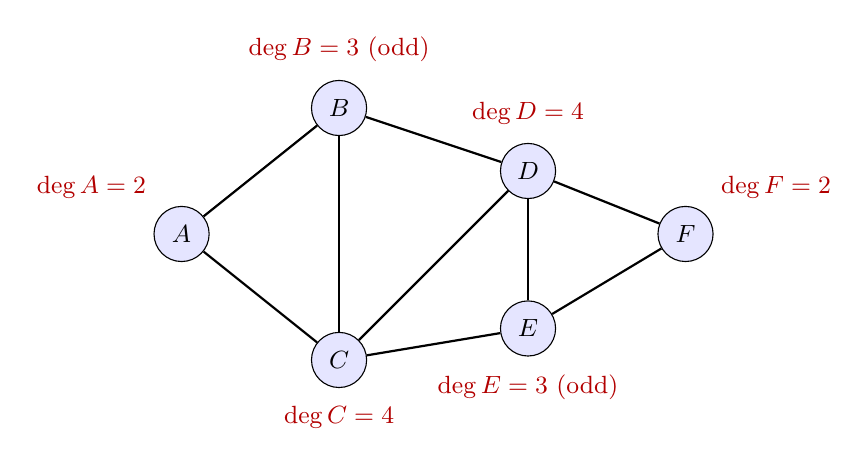
\begin{tikzpicture}[every node/.style={font=\small}, v/.style={draw, circle, fill=blue!10, minimum size=7mm, inner sep=0pt}]
	\node[v] (A) at (0,0) {$A$};
	\node[v] (B) at (2,1.6) {$B$};
	\node[v] (C) at (2,-1.6) {$C$};
	\node[v] (D) at (4.4,0.8) {$D$};
	\node[v] (E) at (4.4,-1.2) {$E$};
	\node[v] (F) at (6.4,0) {$F$};
	\foreach \a/\b in {A/B, A/C, B/C, B/D, C/D, C/E, D/E, D/F, E/F} {\draw[thick] (\a) -- (\b);}
	\node[red!70!black, font=\small, above left=3pt of A] {$\deg A=2$};
	\node[red!70!black, font=\small, above=3pt of B] {$\deg B=3$ (odd)};
	\node[red!70!black, font=\small, below=3pt of C] {$\deg C=4$};
	\node[red!70!black, font=\small, above=3pt of D] {$\deg D=4$};
	\node[red!70!black, font=\small, below=3pt of E] {$\deg E=3$ (odd)};
	\node[red!70!black, font=\small, above right=3pt of F] {$\deg F=2$};
	\end{tikzpicture}
\end{document}
